% !TeX program = pdflatex
\documentclass[11pt,a4paper]{article}

\usepackage[utf8]{inputenc}
\usepackage[T1]{fontenc}
\usepackage[spanish,provide=*]{babel}
\usepackage{amsmath,amssymb}
\usepackage{geometry}
\usepackage{graphicx}
\usepackage{booktabs}
\usepackage{siunitx}
\usepackage{tikz}
\usepackage{caption}
\usepackage[hidelinks]{hyperref}
\usepackage{float}

\geometry{margin=1.5cm}
\graphicspath{{figures/}}

\title{TEMAS SELECTOS DE C\'OMPUTO DE ALTO RENDIMIENTO PARA SIMULACIONES F\'ISICAS\\
Analisis Num\'erico y Computacional\\
Ecuacion de Calor/Laplace en 1D y 2D\\
Dr. Juan Carlos Cajas}
\author{Autor: Emilio Ramirez}
\date{\today}

\begin{document}

\maketitle

\begin{abstract}
Este documento presenta la formulaci\'on matem\'atica, discretizaci\'on por diferencias
finitas y evaluacion computacional de solucionadores para ecuaciones de tipo
calor/Laplace. Se usa el algoritmo de Thomas para sistemas tridiagonales y se
analiza el rendimiento de la paralelizaci\'on con OpenMP en el caso bidimensional.
\end{abstract}

\section{Introducci\'on}
El objetivo es documentar una linea base reproducible para comparar variantes de
implementacion sin cambiar el paradigma matem\'atico ni de paralelizaci\'on.

\section{Modelo matem\'atico}
\subsection{Caso 1D estacionario}
\begin{equation}
\frac{d}{dx}\left(k\frac{dT}{dx}\right) + \dot{q} = 0
\end{equation}

Para $k$ constante (material isotr\'opico y $\Delta T$ peque\~nos) 
y sin fuentes internas ($\dot{q}=0$), se obtiene la Ecuaci\'on de Laplace:

\begin{equation}
\frac{d^2T}{dx^2}=0
\end{equation}

\subsection{Caso 2D estacionario}

Para el caso bidimensional estacionario, se obtiene la ecuaci\'on de Laplace en 2D:

\begin{equation}
\frac{\partial}{\partial x}\left(k\frac{\partial T}{\partial x}\right) + \frac{\partial}{\partial y}\left(k\frac{\partial T}{\partial y}\right) + \dot{q} = 0
\end{equation}

\begin{equation}
\Rightarrow \frac{\partial^2T}{\partial x^2}+\frac{\partial^2T}{\partial y^2}=0
\end{equation}

\begin{equation}
\Rightarrow \nabla^2 T = 0
\end{equation}

\subsection{Condiciones de frontera}

Se consideran condiciones de frontera de tipo Dirichlet (temperatura fija) y 
Neumann (flujo de calor especificado) seg\'un el experimento.

\textbf{Frontera tipo Dirichlet:}

\begin{equation}
T(0)=T_0, \quad T(L)=T_L
\end{equation}

\textbf{Frontera tipo Neumann:}

Si $q_N$ representa el flujo de calor saliente normal a la frontera, la
condici\'on de Neumann se escribe como:

\begin{equation}
-k\nabla T \cdot \mathbf{n} = q_N.
\end{equation}

En el caso unidimensional, con normal exterior $\mathbf{n}=-1$ en $x=0$ y
$\mathbf{n}=1$ en $x=L$, esto equivale a:

\begin{equation}
k\frac{dT}{dx}\bigg|_{x=0} = q_0, \quad
-k\frac{dT}{dx}\bigg|_{x=L} = q_L.
\end{equation}

\section{Discretizacion del caso 1D}

La ecuaci\'on de Laplace se discretiza usando diferencias finitas.

\subsection{Ecuaci\'on interior}

Se parte de la ecuaci\'on diferencial Eq. (2) discretizada:

\begin{equation}
\frac{\Delta}{\Delta x} \left( \frac{\Delta T}{\Delta x} \right) = 0
\end{equation}

\begin{equation}
\Rightarrow \frac{\Delta}{\Delta x} \left( \frac{T(i + 1) - T(i)}{\Delta x} \right) = 0
\end{equation}

\begin{equation}
\Rightarrow\frac{ \Delta T(i + 1) - \Delta T(i)}{ (\Delta x)^2} = 0
\end{equation}

\begin{equation}
\Rightarrow \frac{\left( T(i + 2) - T(i + 1) \right) - 
\left( T(i + 1) - T(i) \right)}{ (\Delta x)^2} = 0
\end{equation}

\begin{equation}
\Rightarrow T_{i+2} - 2 T_{i+1} + T_{i} = 0
\end{equation}

Cambiando el \'indice $i+1 \to i$:

\begin{equation}
T_{i+1} -2T_i + T_{i-1}=0
\end{equation}

con condiciones de frontera de tipo Dirichlet/Neumann seg\'un el experimento.

\textbf{Ecuaci\'on matricial 1D:}

La Eq. (13) se puede escribir en forma matricial $A \mathbf{T} = \mathbf{r}$,
donde $A$ es una matriz tridiagonal con $-2$ en la diagonal principal y $1$ 
en las diagonales adyacentes, $\mathbf{T}$ es el vector de temperaturas 
desconocidas y $\mathbf{r}$ es el vector de condiciones de frontera.

\begin{equation}
\begin{pmatrix}
1 & -2 & 1 & 0 & 0  \cdots & 0 & 0 & 0 \\
0 & 1 & -2 & 1 & 0  \cdots & 0 & 0 & 0 \\
0 & 0 & 1 & -2 & 1  \cdots & 0 & 0 & 0 \\
\vdots & \vdots & \vdots & \ddots & \vdots \\
0 & 0 & 0 & 0 & 0  \cdots & 1 & -2 & 1
\end{pmatrix}
\begin{pmatrix}
T_2 \\
T_3 \\
T_4 \\
\vdots \\
T_{n-1}
\end{pmatrix}
=
\begin{pmatrix}
0 \\
0 \\
0 \\
\vdots \\
0
\end{pmatrix}
\end{equation}

Se hace notar que faltan las temperaturas frontera i.e. $T_1$ y $T_n$ que 
depender\'an del tipo de frontera (Dirichlet o Neumann).

\textbf{Ecuaci\'on matricial 1D con condiciones frontera tipo Dirichlet:}

Con condiciones de frontera de tipo Dirichlet, el sistema se modifica para 
incluir los valores conocidos en las matrices. Dado que $T_1$ y $T_n$ son 
conocidos:

\begin{equation}
T_1 = T_0, \quad T_n = T_L
\end{equation}

\begin{equation}
\begin{pmatrix}
1 & 0 & 0 & 0 & 0  \cdots & 0 & 0 & 0 \\
1 & -2 & 1 & 0 & 0  \cdots & 0 & 0 & 0 \\
0 & 1 & -2 & 1 & 0  \cdots & 0 & 0 & 0 \\
\vdots & \vdots & \vdots & \ddots & \vdots \\
0 & 0 & 0 & 0 & 0  \cdots & 1 & -2 & 1 \\
0 & 0 & 0 & 0 & 0  \cdots & 0 & 0 & 1
\end{pmatrix}
\begin{pmatrix}
T_1 \\
T_2 \\
T_3 \\
\vdots \\
T_{n-1} \\
T_n
\end{pmatrix}
=
\begin{pmatrix}
T_0 \\
0 \\
0 \\
\vdots \\
0 \\
T_L
\end{pmatrix}
\end{equation}

\textbf{Ecuaci\'on matricial 1D con frontera izquierda tipo Neumann:}

Se estudia el caso en el que la frontera izquierda usa una condici\'on de Neumann
y la frontera derecha conserva una condici\'on de Dirichlet. Con flujo saliente
normal $q_0$ en $x=0$:

\begin{equation}
k\frac{dT}{dx}\bigg|_{x=0}=q_0.
\end{equation}

Aproximando la derivada normal con una diferencia hacia adelante:

\begin{equation}
\frac{dT}{dx}\bigg|_{x=0} \approx \frac{T_2-T_1}{\Delta x},
\end{equation}

se obtiene:

\begin{equation}
k\frac{T_2-T_1}{\Delta x}=q_0
\quad \Rightarrow \quad
-T_1+T_2=\frac{q_0}{k} \Delta x
\end{equation}

Por tanto, el sistema algebraico para una frontera izquierda Neumann y una
frontera derecha Dirichlet $T_n=T_L$ queda:

\begin{equation}
\begin{pmatrix}
-1 & 1 & 0 & 0 & 0  \cdots & 0 & 0 & 0 \\
1 & -2 & 1 & 0 & 0  \cdots & 0 & 0 & 0 \\
0 & 1 & -2 & 1 & 0  \cdots & 0 & 0 & 0 \\
\vdots & \vdots & \vdots & \ddots & \vdots \\
0 & 0 & 0 & 0 & 0  \cdots & 1 & -2 & 1 \\
0 & 0 & 0 & 0 & 0  \cdots & 0 & 0 & 1
\end{pmatrix}
\begin{pmatrix}
T_1 \\
T_2 \\
T_3 \\
\vdots \\
T_{n-1} \\
T_n
\end{pmatrix}
=
\begin{pmatrix}
\dfrac{q_0}{k} \Delta x \\
0 \\
0 \\
\vdots \\
0 \\
T_L
\end{pmatrix}.
\end{equation}

Si se imponen condiciones de Neumann en ambos extremos para la ecuaci\'on de
Laplace sin fuentes, el sistema queda determinado solo hasta una constante
aditiva y requiere una condici\'on adicional de referencia. Adem\'as, los flujos
deben cumplir la condici\'on de compatibilidad $q_0+q_L=0$.

\section{Algoritmo de Thomas}

Tenemos el sistema tridiagonal $A \mathbf{T} = \mathbf{r}$, donde $A$ es 
una matriz tridiagonal con elementos $a_i$ en la subdiagonal, $b_i$ en la diagonal,
y $c_i$ en la superdiagonal. De la misma manera, $\mathbf{T}$ es el vector de 
temperaturas desconocidas y $\mathbf{r}$ es el vector de condiciones de frontera,
con elementos $d_i$.

\begin{align*}
b_1 T_1 + c_1 T_2 &= r_1 \\
a_2 T_1 + b_2 T_2 + c_2 T_3 &= r_2 \\
a_3 T_2 + b_3 T_3 + c_3 T_4 &= r_3 \\
&\vdots \\
a_{n-1} T_{n-2} + b_{n-1} T_{n-1} + c_{n-1} T_n &= r_{n-1} \\
a_n T_{n-1} + b_n T_n &= r_n
\end{align*}

\begin{equation}
\begin{pmatrix}
b_1 & c_1 & 0 & 0 & 0  \cdots & 0 & 0 & 0 \\
a_2 & b_2 & c_2 & 0 & 0  \cdots & 0 & 0 & 0 \\
0 & a_3 & b_3 & c_3 & 0  \cdots & 0 & 0 & 0 \\
\vdots & \vdots & \vdots & \ddots & \vdots \\
0 & 0 & 0 & 0 & 0  \cdots & a_{n-1} & b_{n-1} & c_{n-1} \\
0 & 0 & 0 & 0 & 0  \cdots & 0 & a_n & b_n
\end{pmatrix}
\begin{pmatrix}T_1 \\
T_2 \\
T_3 \\
\vdots \\
T_{n-1} \\
T_n
\end{pmatrix}
=
\begin{pmatrix}r_1 \\
r_2 \\
r_3 \\
\vdots \\
r_{n-1} \\
r_n
\end{pmatrix}
\end{equation}

As\'i, se tienen las ecuaciones del sistema tridiagonal a resolver:

\begin{equation}
a_i T_{i-1}+b_iT_i+c_iT_{i+1}=r_i,
\quad i=1,2,\ldots,n, \quad a_1=0, \quad c_n=0.
\end{equation}

Resolviendo,

\begin{equation}
T_1 = \frac{r_1 - c_1 T_2}{b_1}
\end{equation}

Y definimos,

\begin{equation}
\tilde{r}_1 = \frac{r_1}{b_1}, \quad \tilde{c}_1 = \frac{c_1}{b_1}
\label{eq:tri_factor_init1}
\end{equation}

Con lo cual, la primera ecuaci\'on se reescribe como:

\begin{equation}
T_1 = \tilde{r}_1 - \tilde{c}_1 T_2
\end{equation}

Si ahora resolvemos el segundo rengl\'on para $T_2$:

\begin{equation}
T_2 = \frac{r_2 - a_2 T_1 - c_2 T_3}{b_2}
\end{equation}

\begin{equation}
\Rightarrow T_2 = \frac{r_2 - a_2 (\tilde{r}_1 - \tilde{c}_1 T_2) - c_2 T_3}{b_2}
\end{equation}

\begin{equation}
\Rightarrow T_2 \left(1 - \frac{a_2 \tilde{c}_1}{b_2}\right) = \frac{r_2 - a_2 \tilde{r}_1 - c_2 T_3}{b_2}
\end{equation}

\begin{equation}
\Rightarrow T_2 = \frac{r_2 - a_2 \tilde{r}_1 - c_2 T_3}{b_2 - a_2 \tilde{c}_1}
\end{equation}

Y si ahora definimos 

\begin{equation}
\tilde{r}_2 = \frac{r_2 - a_2 \tilde{r}_1}{b_2 - a_2 \tilde{c}_1}, \quad 
\tilde{c}_2 = \frac{c_2}{b_2 - a_2 \tilde{c}_1}
\label{eq:tri_factor_init2}
\end{equation}

Entonces nos queda,

\begin{equation}
T_2 = \tilde{r}_2 - \tilde{c}_2 T_3
\end{equation}

En general, para $i=2,3,\ldots,n-1$ se tiene:

\begin{equation}
T_i = \tilde{r}_i - \tilde{c}_i T_{i+1},
\end{equation}

con:

\begin{equation}
\tilde{r}_i = \frac{r_i - a_i \tilde{r}_{i-1}}{b_i - a_i \tilde{c}_{i-1}}, \quad
\tilde{c}_i = \frac{c_i}{b_i - a_i \tilde{c}_{i-1}}
\label{eq:tri_solve_general}
\end{equation}

Para $T_n$ se tiene:

\begin{equation}
T_n = \frac{r_n - a_n T_{n-1}}{b_n}
\label{eq:tri_solve_last}
\end{equation}

\begin{equation}
\Rightarrow T_n = \frac{r_n - a_n 
\left( \tilde{r}_{n-1} - \tilde{c}_{n-1} T_{n} \right)}{b_n}
\end{equation}

\begin{equation}
\Rightarrow T_n \left(1 - \frac{a_n \tilde{c}_{n-1}}{b_n}\right) 
= \frac{r_n - a_n \tilde{r}_{n-1}}{b_n}
\end{equation}

\begin{equation}
\Rightarrow T_n = \frac{r_n - a_n \tilde{r}_{n-1}}{b_n - a_n \tilde{c}_{n-1}}
\end{equation}

\begin{equation}
\Rightarrow T_n = \tilde{r}_n
\label{eq:tri_solve_last_final}
\end{equation}

Conociendo $T_n$, se obtiene $T_{n-1}$, luego $T_{n-2}$, y as\'i sucesivamente 
hasta $T_1$.

\medskip

Como ejemplo, se muestra un peque\~no caso de una frontera izquierda Neumann 
con flujo $q_0$ y una frontera derecha Dirichlet con temperatura $T_L = 0$. 
Para $n = 5$ y una longitud $L = 10 \text{ m}$, los coeficientes de la matriz tridiagonal y el vector de 
resultados son:

\begin{equation}
A = \begin{pmatrix}
  -1 & 1 & 0 & 0 & 0 \\
  1 & -2 & 1 & 0 & 0 \\
  0 & 1 & -2 & 1 & 0 \\
  0 & 0 & 1 & -2 & 1 \\
  0 & 0 & 0 & 0 & 1
\end{pmatrix}, \quad
\mathbf{r} = \begin{pmatrix}
\frac{q_0}{k} \Delta x\\
0 \\
0 \\
0 \\
0
\end{pmatrix}
\end{equation}

Tenemos entonces, estableciendo que $q_0/k = -1\textrm{.}0$ K/m y 
$\Delta x = \frac{L}{n - 1} = \frac{10 \text{ m}}{5 - 1} = 2\textrm{.}5 \text{ m}$:

\begin{equation}
  \begin{array}{l}
    a_1 = 0 \\
    a_2 = 1 \\
    a_3 = 1 \\
    a_4 = 1 \\
    a_5 = 0
  \end{array} \quad
  \begin{array}{l}
    b_1 = -1 \\
    b_2 = -2 \\
    b_3 = -2 \\
    b_4 = -2 \\
    b_5 = 1
  \end{array} \quad
  \begin{array}{l}
    c_1 = 1 \\
    c_2 = 1 \\
    c_3 = 1 \\
    c_4 = 1 \\
    c_5 = 0
  \end{array} \quad 
  \begin{array}{l}
    r_1 = \frac{q_0}{k} \Delta x = -2\textrm{.}5\\
    r_2 = 0 \\
    r_3 = 0 \\
    r_4 = 0 \\
    r_5 = 0
  \end{array}
\end{equation}

Con estos valores podemos calcular los coeficientes modificados $\tilde{c}_i$ y 
el lado derecho modificado $\tilde{r}_i$ para el algoritmo de Thomas:

\begin{equation}
\begin{array}{l}
\tilde{c}_1 = \frac{c_1}{b_1} = -1 \\
\tilde{c}_2 = \frac{c_2}{b_2 - a_2 \tilde{c}_1} = \frac{1}{-2 - 1(-1)} = -1 \\
\tilde{c}_3 = \frac{c_3}{b_3 - a_3 \tilde{c}_2} = \frac{1}{-2 - 1(-1)} = -1 \\
\tilde{c}_4 = \frac{c_4}{b_4 - a_4 \tilde{c}_3} = \frac{1}{-2 - 1(-1)} = -1 \\
\tilde{c}_5 = \frac{c_5}{b_5 - a_5 \tilde{c}_4} = 0
\end{array} \quad
\begin{array}{l}
\tilde{r}_1 = \frac{r_1}{b_1} = 2\textrm{.}5 \\
\tilde{r}_2 = \frac{r_2 - a_2 \tilde{r}_1}{b_2 - a_2 \tilde{c}_1} = \frac{0 - 1(2\textrm{.}5)}{-2 - 1(-1)} = 2\textrm{.}5 \\
\tilde{r}_3 = \frac{r_3 - a_3 \tilde{r}_2}{b_3 - a_3 \tilde{c}_2} = \frac{0 - 1(2\textrm{.}5)}{-2 - 1(-1)} = 2\textrm{.}5 \\
\tilde{r}_4 = \frac{r_4 - a_4 \tilde{r}_3}{b_4 - a_4 \tilde{c}_3} = \frac{0 - 1(2\textrm{.}5)}{-2 - 1(-1)} = 2\textrm{.}5 \\
\tilde{r}_5 = \frac{r_5 - a_5 \tilde{r}_4}{b_5 - a_5 \tilde{c}_4} = 0
\end{array}
\end{equation}

Y ahora podemos resolver hacia atr\'as para obtener las temperaturas:

\begin{equation}
\begin{array}{l}
T_5 = \tilde{r}_5 = 0 \\
T_4 = \tilde{r}_4 - \tilde{c}_4 T_5 = 2\textrm{.}5 - (-1)(0) = 2\textrm{.}5 \\
T_3 = \tilde{r}_3 - \tilde{c}_3 T_4 = 2\textrm{.}5 - (-1)(2\textrm{.}5) = 5 \\
T_2 = \tilde{r}_2 - \tilde{c}_2 T_3 = 2\textrm{.}5 - (-1)(5) = 7\textrm{.}5 \\
T_1 = \tilde{r}_1 - \tilde{c}_1 T_2 = 2\textrm{.}5 - (-1)(7\textrm{.}5) = 10
\end{array}
\end{equation}
Por lo tanto, la soluci\'on del sistema es:
\begin{equation}
\mathbf{T} = \begin{pmatrix}
10 \\
7\textrm{.}5 \\
5 \\
2\textrm{.}5 \\
0
\end{pmatrix}
\end{equation}

A continuaci\'on se muestra la implementaci\'on en Fortran del algoritmo de 
Thomas para resolver el sistema tridiagonal resultante de la discretizaci\'on 
de la ecuaci\'on de Laplace en 1D.

\section{Metodolog\'ia computacional del caso 1D}

Para el caso unidimensional se resuelve directamente el sistema tridiagonal
producido por la discretizaci\'on de Laplace:

\begin{equation}
A\mathbf{T}=\mathbf{r}.
\end{equation}

Se implementa el algoritmo de Thomas para resolver este sistema de forma 
eficiente. Se usa el comando \verb|gfortran tridiagonal.f90 calor1D.f90 -o calor1D| 
para compilar la versi\'on secuencial. El programa se ejecuta con \verb|./calor1D| 
y los resultados se guardan en archivos de texto para su posterior an\'alisis.

\medskip{}

Se muestra a continuaci\'on el c\'odigo Fortran de la versi\'on secuencial 
para el caso 1D. Se comienza abriendo el programa y declarando las variables 
necesarias para el algoritmo:

\begin{verbatim}
Program Calor1D
  !
  Implicit none
  !
  ! Declaracion de variables
  !
  ! Iteradores y tamaño del problema
  !
  integer :: ii
  integer, parameter :: L = 10 ! metros
  integer, parameter :: nn = 60
  double precision, parameter :: q0_sobre_k = -1.d0
  !
  ! Variables del dominio computacional
  !
  double precision :: deltax
  !
  ! Variables del problema f\'isico
  !
  ! double precision :: aa(nn,nn) ! matriz para el problema algebraico
  double precision :: tt(nn)    ! vector de inc\'ognitas
  double precision :: rr(nn)    ! vector de resultados del s. ecuaciones
  !
  double precision :: aa(nn), bb(nn), cc(nn) ! Variables para almacenar
                                             ! las diagonales de la matriz tridiagonal
  double precision :: cp(nn), den(nn)
\end{verbatim}

Establecemos el dominio computacional y el paso de malla $ \Delta x = L/(nn - 1)$:
El valor $L=10$ metros define la longitud total del dominio de soluci\'on; se elige
arbitrariamente para este problema de prueba. La discretizaci\'on se realiza 
con $nn=60$ nodos (59 dominios), resultando en $ \Delta x = L/(nn-1) = 10/59 $

\begin{verbatim}
  ! Dominio computacional
  deltax  = dble(L)/(nn-1)
\end{verbatim}

Luego, se inicializan los vectores necesarios para el algoritmo de Thomas.
Se hace notar que no se construye la matriz completa $A$, sino que se almacenan 
solamente las diagonales $a$, $b$ y $c$ en los vectores correspondientes.

\begin{verbatim}
  ! Inicializacion de variables
  !
  aa(:)   = 0.d0
  bb(:)   = 0.d0
  cc(:)   = 0.d0
  rr(:)   = 0.d0
\end{verbatim}

Se ensamblan los coeficientes de la matriz tridiagonal y el vector de resultados
seg\'un la discretizaci\'on de la ecuaci\'on de Laplace. Para los nodos 
interiores, los coeficientes son constantes: $a_i=1$, $b_i=-2$ y $c_i=1$.

\begin{verbatim}
  ! Ensamblar la matriz tridiagonal y el vector de resultados
  do ii = 2, nn-1
     !
     aa(ii) = 1.d0
     bb(ii) =-2.d0
     cc(ii) = 1.d0
     rr(ii) = 0.d0
     !
  end do
\end{verbatim}

A continuaci\'on, se imponen las condiciones de frontera. En este caso, 
se asume una condici\'on de Neumann en el extremo izquierdo ($x=0$) con un 
flujo tal que  $q_0 / k = -1\textrm{.}0$ K/m, y una condici\'on de 
Dirichlet en el extremo derecho ($x=L$) 
con temperatura $T_L=0$. Esto se traduce en los coeficientes de la primera y 
\'ultima ecuaciones del sistema.

\begin{verbatim}
  ! Impone cond. frontera
  !
  aa(1)     = 0.d0 ! no se usa en los c'alculos
  bb(1)     =-1.d0
  cc(1)     = 1.d0
  rr(1)     = q0_sobre_k * deltax
  !  
  aa(nn)    = 0.d0
  bb(nn)    = 1.d0
  cc(nn)    = 0.d0 ! no se usa en los c'alculos
  rr(nn)    = 0.d0 
\end{verbatim}

Se resuelve el sistema tridiagonal usando el algoritmo de Thomas, que se 
implementa en las subrutinas \verb|tri_factor| y \verb|tri_solve|. Estas
subrutinas realizan la factorizaci\'on y la resoluci\'on del sistema de 
forma eficiente, aprovechando la estructura tridiagonal de la matriz.

\begin{verbatim}
  ! Resolver el problema algebraico
  !
  call tri_factor(aa,bb,cc,cp,den,nn)
  call tri_solve(aa,cp,den,rr,tt,nn)
\end{verbatim}

Finalmente, se guarda el resultado en un archivo de texto para su posterior
an\'alisis. Se escribe el vector de temperaturas $tt$ junto con las posiciones
correspondientes en el dominio.

\begin{verbatim}
  ! Postproceso
  !
  do ii = 1, nn
     write(101,*) (ii-1)*deltax, tt(ii)
  end do
  !
end Program Calor1D
\end{verbatim}

\textbf{Subrutina \texttt{tri}}  

\medskip

La subrutina \verb|tri| es adicional y no se usa para la resoluci\'on del 
sistema tridiagonal, pero se incluye para ilustrar el proceso de 
eliminaci\'on gaussiana y sustituci\'on hacia atr\'as.

\begin{verbatim}
subroutine tri(a,b,c,r,u,nn)
  !
  ! Subrutina que resuelve el problema usando eliminaci\'on gaussiana
  !
  ! Ax=r donde A es una matriz tridiagonal con elementos a, b, c
  ! y devuelve el valor de u
  !
  implicit none
  !
  integer,          intent(in)    :: nn
  double precision, intent(in)    :: a(nn),c(nn)
  double precision, intent(inout) :: b(nn),r(nn)
  double precision, intent(inout) :: u(nn)
  integer :: ii
  double precision :: m
\end{verbatim}

Para el barrido hacia adelante se usa \textit{(\texttt{gausselim}):}
Para $i = 2, 3, \ldots, n$, se calcula el multiplicador de eliminaci\'on y
se actualizan la diagonal y el lado derecho \textit{in-place}:

\begin{align}
m_{i}          &= \frac{a_{i}}{b_{i-1}}, \\
b_{i}^{*}          &\leftarrow b_{i} - m_{i}\, c_{i-1}, \\
r_{i}^{*}          &\leftarrow r_{i} - m_{i}\, r_{i-1}.
\end{align}

\begin{verbatim}
  ! Eliminaci\'on elementos bajo la matriz
  gausselim: do ii=2,nn
     m = a(ii)/b(ii-1)
     r(ii)=r(ii)-m*r(ii-1)
     b(ii)=b(ii)-m*c(ii-1)
  end do gausselim
  !
\end{verbatim}

Tras este barrido el sistema original $A\mathbf{u}=\mathbf{r}$ ha quedado
reducido a uno triangular superior equivalente $U\mathbf{u}=\mathbf{r}^*$,
donde $\mathbf{r}^*$ denota el lado derecho transformado.

\medskip

Sustituci\'on hacia atr\'as \textit{(\texttt{sustatras}):}
Se obtiene la \'ultima inc\'ognita directamente y luego se retrocede:

\begin{align}
u_{n} &= \frac{r_{n}^{\,*}}{b_{n}^{\,*}}, \\[4pt]
u_{i} &= \frac{r_{i}^{\,*} - c_{i}\, u_{i+1}}{b_{i}^{\,*}},
\quad i = n-1,\, n-2,\, \ldots,\, 1.
\end{align}

\begin{verbatim}
  ! Soluci\'on para u
  !
  u(nn)=r(nn)/b(nn)
  sustatras: do ii=nn-1,1,-1
     u(ii)=(r(ii)-c(ii)*u(ii+1))/b(ii)
  end do sustatras
  !
end subroutine tri
\end{verbatim}

El coste total tambi\'en es $\mathcal{O}(n)$ operaciones, frente a los
$\mathcal{O}(n^3)$ de una eliminaci\'on gaussiana general. Se declara esta
subrutina para ilustrar el proceso completo, aunque en la implementaci\'on
final se opta por usar las subrutinas \verb|tri_factor| y \verb|tri_solve|
que realizan la factorizaci\'on y la resoluci\'on de forma separada.

\medskip

\textbf{Subrutina \texttt{tri\_factor}:}

\medskip

Se explica a continuaci\'on el c\'odigo de la subrutina \verb|tri_factor|, 
que realiza la factorizaci\'on de Thomas para una matriz tridiagonal 
constante.

\medskip

Se declaran las variables de entrada y salida, incluyendo los vectores de 
coeficientes de la matriz tridiagonal y los vectores para almacenar la 
factorizaci\'on.

\begin{verbatim}
subroutine tri_factor(a,b,c,cp,den,nn)
  !
  ! Factorizacion de Thomas para una matriz tridiagonal constante.
  !
  implicit none
  !
  integer,          intent(in)  :: nn
  double precision, intent(in)  :: a(nn),b(nn),c(nn)
  double precision, intent(out) :: cp(nn),den(nn)
  integer :: ii
\end{verbatim}

Se inicializan los vectores de la factorización seg\'un las ecuaciones 
\ref{eq:tri_factor_init1} y \ref{eq:tri_factor_init2}:

\begin{verbatim}
  den(1) = b(1)
  cp(1)  = c(1)/den(1) ! cp \equiv c'

  do ii=2,nn-1
     den(ii) = b(ii) - a(ii)*cp(ii-1)
     cp(ii) = c(ii)/den(ii)
  end do
  den(nn) = b(nn) - a(nn)*cp(nn-1)
  cp(nn) = 0.d0
end subroutine tri_factor
\end{verbatim}

\textbf{Subrutina \texttt{tri\_solve}:}

\medskip

Se muestra a continuaci\'on el c\'odigo de la subrutina \verb|tri_solve|, que
realiza la sustituci\'on hacia atr\'as para resolver el sistema tridiagonal
usando la factorizaci\'on calculada por \verb|tri_factor|.

\begin{verbatim}
subroutine tri_solve(a,cp,den,r,u,nn)
  !
  ! Sustituci\'on usando la factorizacion calculada por tri_factor.
  ! Modifica r in-place para guardar el lado derecho transformado.
  !
  implicit none
  !
  integer,          intent(in)    :: nn
  double precision, intent(in)    :: a(nn),cp(nn),den(nn)
  double precision, intent(inout) :: r(nn)
  double precision, intent(inout) :: u(nn)
  integer :: ii
\end{verbatim}

Se realiza el barrido hacia adelante seg\'un la ecuaci\'on 
\ref{eq:tri_solve_general} para transformar el lado derecho usando la
factorizaci\'on calculada.

\begin{verbatim}
  r(1) = r(1)/den(1)
  do ii=2,nn
     r(ii) = (r(ii) - a(ii)*r(ii-1))/den(ii)
  end do
\end{verbatim}

Finalmente, usando las ecuaciones \ref{eq:tri_solve_last} y 
\ref{eq:tri_solve_last_final}, se obtiene el vector de temperaturas $u$ 
mediante sustituci\'on hacia atr\'as.

\begin{verbatim}
  u(nn) = r(nn)
  do ii=nn-1,1,-1
     u(ii) = r(ii) - cp(ii)*u(ii+1)
  end do
end subroutine tri_solve
\end{verbatim}

\textbf{Resultados}

Se muestran a continuaci\'on los resultados obtenidos para el caso 1D, 
incluyendo la distribuci\'on de temperatura a lo largo del dominio de 
soluci\'on. Se observa que la temperatura disminuye linealmente desde el 
extremo izquierdo, donde se impone un flujo de calor, hasta el extremo derecho, 
donde se fija la temperatura a cero.

\begin{figure}[h]
\centering
\includegraphics[width=0.8\textwidth]{figures/secuencial/calor1D/temperatura_1d.png}
\caption{Distribución de temperatura en el caso 1D}
\label{fig:temp_1d}
\end{figure}

\section{Discretizaci\'on del caso 2D}

En el caso bidimensional, la ecuaci\'on de Laplace se discretiza como:

\begin{equation}
\label{eq:laplace_2d}
\frac{T_{i+1,j}-2T_{i,j}+T_{i-1,j}}{(\Delta x)^2}
+
\frac{T_{i,j+1}-2T_{i,j}+T_{i,j-1}}{(\Delta y)^2}
=0.
\end{equation}

Separando los t\'erminos en la direcci\'on $x$:

\begin{equation}
\label{eq:laplace_2d_separated}
\frac{1}{(\Delta x)^2}T_{i-1,j}
-2\left(\frac{1}{(\Delta x)^2}+\frac{1}{(\Delta y)^2}\right)T_{i,j}
+\frac{1}{(\Delta x)^2}T_{i+1,j}
=-\frac{T_{i,j-1}+T_{i,j+1}}{(\Delta y)^2}.
\end{equation}

Esta expresi\'on genera un sistema tridiagonal por cada linea horizontal
$j$:

\begin{equation}
a_i^{(x)}T_{i-1,j}+b_i^{(x)}T_{i,j}+c_i^{(x)}T_{i+1,j}=r_i^{(x)}.
\end{equation}

Los coeficientes usados son:

\begin{align}
a_i^{(x)} &= \frac{1}{(\Delta x)^2}, \label{eq:coef_tridiagonal_x_2D_a} \\
b_i^{(x)} &= -2\left(\frac{1}{(\Delta x)^2}+\frac{1}{(\Delta y)^2}\right), \label{eq:coef_tridiagonal_x_2D_b} \\
c_i^{(x)} &= \frac{1}{(\Delta x)^2}, \label{eq:coef_tridiagonal_x_2D_c} \\
r_i^{(x)} &= -\frac{T_{i,j-1}+T_{i,j+1}}{(\Delta y)^2}.
\label{eq:coef_tridiagonal_x_2D_r}
\end{align}

De forma an\'aloga, separando los t\'erminos en la direcci\'on $y$:

\begin{equation}
\frac{1}{(\Delta y)^2}T_{i,j-1}
-2\left(\frac{1}{(\Delta x)^2}+\frac{1}{(\Delta y)^2}\right)T_{i,j}
+\frac{1}{(\Delta y)^2}T_{i,j+1}
=-\frac{T_{i-1,j}+T_{i+1,j}}{(\Delta x)^2}.
\end{equation}

Esto produce sistemas tridiagonales verticales:

\begin{equation}
a_j^{(y)}T_{i,j-1}+b_j^{(y)}T_{i,j}+c_j^{(y)}T_{i,j+1}=r_j^{(y)},
\end{equation}

con:

\begin{align}
a_j^{(y)} &= \frac{1}{(\Delta y)^2}, \label{eq:coef_tridiagonal_y_2D_a} \\
b_j^{(y)} &= -2\left(\frac{1}{(\Delta x)^2}+\frac{1}{(\Delta y)^2}\right), \label{eq:coef_tridiagonal_y_2D_b} \\
c_j^{(y)} &= \frac{1}{(\Delta y)^2}, \label{eq:coef_tridiagonal_y_2D_c} \\
r_j^{(y)} &= -\frac{T_{i-1,j}+T_{i+1,j}}{(\Delta x)^2}.
\label{eq:coef_tridiagonal_y_2D_r}
\end{align}

El proceso iterativo se detiene cuando el cambio entre dos iteraciones
consecutivas es menor que una tolerancia prescrita. El residuo usado es:

\begin{equation}
R^{(k)}=
\left[
\sum_{i=1}^{n_x}\sum_{j=1}^{n_y}
\left(T_{i,j}^{(k)}-T_{i,j}^{(k-1)}\right)^2
\right]^{1/2}.
\end{equation}

El criterio de convergencia es:

\begin{equation}
R^{(k)}<\varepsilon.
\end{equation}

Se usa como ejemplo una placa bidimensional con dimensiones $L_x=8$ m y 
$L_y=4$ m, discretizada con $n_x=5$ nodos en la direcci\'on $x$ y $n_y=3$ nodos 
en la direcci\'on $y$. Se imponen condiciones de frontera de Dirichlet en los
extremos izquierdo y derecho con temperaturas $T_0=0^{o}C$ y $T_{L_x}=10^{o}C$, 
mientras que en los extremos superior e inferior se imponen condiciones de 
Neumann con flujo de calor $q_0/k= 0$ K/m.

\begin{figure}[h]
\centering
\captionsetup{justification=centering}
\makebox[\textwidth][c]{%
\begin{tikzpicture}[scale=1.5]
  % Draw the plate
  \draw[thick] (0,0) rectangle (8,4);

  % Draw grid lines
  \foreach \j in {0,2,4} {
    \draw[thin,dashed] (0,\j) -- (8,\j);
  }
  \foreach \i in {0,2,4,6,8} {
    \draw[thin,dashed] (\i,0) -- (\i,4);
  }
  
  % Draw grid nodes
  \foreach \i in {0,2,4,6,8} {
    \foreach \j in {0,2,4} {
      \fill (\i,\j) circle (2pt);
    }
  }
  
  % Label dimensions
  \draw[<->,>=stealth] (-0.3,0) -- (-0.3,4);
  \node at (-1.0,1.5) {\textbf{$L_y=4$ m}};
  
  \draw[<->,>=stealth] (0,-0.3) -- (8,-0.3);
  \node at (4,-0.8) {\textbf{$L_x=8$ m}};
  
  % Label boundary conditions
  \node[black,left] at (-0.5,2) {\small $T_0=0^{\circ}\mathrm{C}$};
  \node[black,right] at (8.1,2) {\small $T_{L_x}=10^{\circ}\mathrm{C}$};
  \node[black,above] at (4,4.2) {\small $q_0/k=0$ K/m};
  \node[black,below] at (4,-0.3) {\small $q_0/k=0$ K/m};
  
  % Mark specific nodes for grid
  \node[below] at (0,-0.5) {$(i,j)$};
  
\end{tikzpicture}
}
\caption{Placa bidimensional discretizada con $n_x=5$ nodos 
en dirección $x$ y $n_y=3$ nodos en dirección $y$. Condiciones de frontera: 
Dirichlet en los extremos izquierdo y derecho, Neumann en los extremos 
superior e inferior.}
\label{fig:placa_2d}
\end{figure}

Se construyen las matrices tridiagonales para cada cada direcci\'on, una 
matriz para cada conjunto de nodos. As\'i en total, se resuelven $n_y$ 
sistemas tridiagonales en la direcci\'on $x$ y $n_x$ sistemas tridiagonales en 
la direcci\'on $y$. En este caso, 3 + 5 = 8 sistemas tridiagonales en total.

\medskip

Dado que los coeficientes de los sistemas tridiagonales se mantendr\'an constantes
en cada iteraci\'on, pues no dependen de las tmeperaturas, se pueden 
pre-calcular los coeficientes modificados para el algoritmo de Thomas antes 
de iniciar las iteraciones. Esto optimiza el proceso de resoluci\'on de los 
sistemas tridiagonales en cada iteraci\'on, ya que se evita recalcular los 
coeficientes en cada paso. Teniendo en cuenta que $\Delta x = L_x/(n_x - 1) = 2$
y $\Delta y = L_y/(n_y - 1) = 2$, los coeficientes de los sistemas tridiagonales 
para cada dirección se establecen como sigue:

\begin{equation}
\begin{array}{@{}l@{\qquad}l@{\qquad}l@{}}
a_1^{(x)} = 0, &
b_1^{(x)} = 1, &
c_1^{(x)} = 0, \\[0.6em]
a_i^{(x)} = \frac{1}{(\Delta x)^2} = 0.25, &
b_i^{(x)} = -2\left(\frac{1}{(\Delta x)^2}+\frac{1}{(\Delta y)^2}\right) = -1, &
c_i^{(x)} = \frac{1}{(\Delta x)^2} = 0.25, \qquad i \in \left\{ 2, 3, 4 \right\} \\[0.6em]
a_{5}^{(x)} = 0, &
b_{5}^{(x)} = 1, &
c_{5}^{(x)} = 0
\end{array}
\end{equation}

\bigskip

\begin{equation}
\begin{array}{@{}l@{\qquad}l@{\qquad}l@{}}
a_1^{(y)} = 0, &
b_1^{(y)} = -1, &
c_1^{(y)} = 1, \\[0.6em]
a_j^{(y)} = \frac{1}{(\Delta y)^2} = 0.25, &
b_j^{(y)} = -2\left(\frac{1}{(\Delta x)^2}+\frac{1}{(\Delta y)^2}\right) = -1, &
c_j^{(y)} = \frac{1}{(\Delta y)^2} = 0.25, \\[0.6em]
a_{n}^{(y)} = -1, &
b_{n}^{(y)} = 1, &
c_{n}^{(y)} = 0
\end{array}
\end{equation}

A continuaci\'on se realiza la factorizaci\'on de Thomas para cada eje:

\begin{equation}
\begin{array}{@{}l@{\qquad}l@{\qquad}l@{}}
\tilde{c}_1^{(x)} = \frac{c_1^{(x)}}{b_1^{(x)}} = 0, 
& \tilde{c}_1^{(y)} = \frac{c_1^{(y)}}{b_1^{(y)}} = -1, \\[0.6em]
\tilde{c}_2^{(x)} = \frac{c_2^{(x)}}{b_2^{(x)} - a_2^{(x)} \tilde{c}_1^{(x)}}
 = \frac{0.25}{-1 - 0.25*0} = -1/4, 
& \tilde{c}_2^{(y)} = \frac{c_2^{(y)}}{b_2^{(y)} - a_2^{(y)} \tilde{c}_1^{(y)}}
 = \frac{0.25}{-1 - 0.25*(-1)} = -1/3, \\[0.6em]
\tilde{c}_3^{(x)} = \frac{c_3^{(x)}}{b_3^{(x)} - a_3^{(x)} \tilde{c}_2^{(x)}}
 = \frac{0.25}{-1 - 0.25*(-0.25)} = -4/15,
& \tilde{c}_3^{(y)} = 0, \\[0.6em]
\tilde{c}_4^{(x)} = \frac{c_4^{(x)}}{b_4^{(x)} - a_4^{(x)} \tilde{c}_3^{(x)}}
 = \frac{0.25}{-1 - 0.25*(-4/15)} = -15/56,
& \\[0.6em]
\tilde{c}_5^{(x)} = 0 &  
\end{array}
\end{equation}

Seguidamente, se imponen las condiciones de frontera:

\begin{equation}
  \texttt{cfx} = \begin{pmatrix}
    0 & 10 \\
    0 & 10 \\
    0 & 10
\end{pmatrix} _{3 \times 2} \qquad 
  \texttt{cfy} = \begin{pmatrix}
    0 & 0 \\
    0 & 0 \\
    \vdots & \vdots \\
    0 & 0
\end{pmatrix} _{5 \times 2}
\end{equation}

Con las condiciones iniciales establecidas, se resuelven los sistemas 
tridiagonales iterativamente. Se comienza con un barrido a lo largo del eje 
\texttt{y} y luego a lo largo del eje \texttt{x}, actualizando las temperaturas 
en cada iteraci\'on. En este paso se est\'a resolviendo la segunda horizontal de
la malla (\(j=2\)) durante el barrido en direcci\'on \(x\).

\begin{center}
\begin{minipage}[c]{0.38\textwidth}
\centering
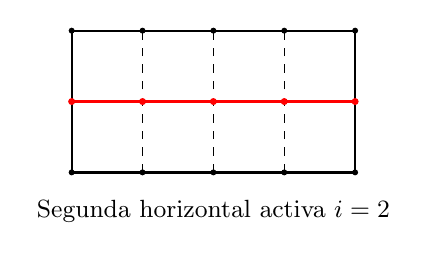
\begin{tikzpicture}[scale=0.45]
  % Malla 5x3 del ejemplo
  \draw[thick] (0,0) rectangle (8,4);
  \foreach \j in {0,2,4} {
    \draw[thin,dashed] (0,\j) -- (8,\j);
  }
  \foreach \i in {0,2,4,6,8} {
    \draw[thin,dashed] (\i,0) -- (\i,4);
  }

  % Fila activa j=2 resaltada
  \draw[very thick,red] (0,2) -- (8,2);

  \foreach \i in {0,2,4,6,8} {
    \foreach \j in {0,2,4} {
      \fill (\i,\j) circle (2.4pt);
    }
  }
  \foreach \i in {0,2,4,6,8} {
    \fill[red] (\i,2) circle (2.8pt);
  }

  \node[below] at (4,-0.5) {\small Segunda horizontal activa \(i=2\)};
\end{tikzpicture}
\end{minipage}
\hfill
\begin{minipage}[c]{0.58\textwidth}
\begin{equation}
\begin{aligned}
r_1^{(x)} &= \texttt{cfx}(2,1) = 0,\\
r_2^{(x)} &= - \frac{1}{(\Delta y)^2} \left( T(2,1) + T(2,3) \right) 
= - \frac{(0+0)}{(\Delta y)^2} = 0,\\
r_3^{(x)} &= - \frac{1}{(\Delta y)^2} \left( T(3,1) + T(3,3) \right) = 0,\\
r_4^{(x)} &= - \frac{1}{(\Delta y)^2} \left( T(4,1) + T(4,3) \right) = 0,\\
r_5^{(x)} &= \texttt{cfx}(2,2) = 10
\end{aligned}
\end{equation}
\end{minipage}
\end{center}

Para este ejemplo reducido, en la primera iteraci\'on se parte de
\(T_{i,j}^{(0)}=0\), con \(\Delta x=\Delta y=2\) y por tanto
\(1/(\Delta x)^2=1/(\Delta y)^2=0.25\). Como \(\texttt{cfx}(2,1)=0\) y
\(\texttt{cfx}(2,2)=10\), el sistema en \(x\) para \(j=2\) queda con:

\begin{equation}
\mathbf{r}^{(x)} = [0,0,0,0,10]^T.
\end{equation}

Se resuelve con Thomas en forma expl\'icita. Para la direcci\'on \(x\), los
coeficientes son:

\begin{equation}
\begin{aligned}
a^{(x)} &= [0,\;0.25,\;0.25,\;0.25,\;0],\\
b^{(x)} &= [1,\;-1,\;-1,\;-1,\;1],\\
c^{(x)} &= [0,\;0.25,\;0.25,\;0.25,\;0].
\end{aligned}
\end{equation}

La factorizaci\'on (ya calculada antes) produce:

\begin{equation}
\begin{aligned}
\tilde c_1^{(x)}&=0, \quad \tilde c_2^{(x)}=-\frac14, \quad
\tilde c_3^{(x)}=-\frac{4}{15}, \quad \tilde c_4^{(x)}=-\frac{15}{56}, \quad
\tilde c_5^{(x)}=0,\\
d_1^{(x)}&=1,\; d_2^{(x)}=-1,\; d_3^{(x)}=-\frac{15}{16},\;
d_4^{(x)}=-\frac{14}{15},\; d_5^{(x)}=1.
\end{aligned}
\end{equation}

En la sustituci\'on hacia adelante sobre \(\mathbf r^{(x)}\):

\begin{equation}
\begin{aligned}
\hat r_1 &= \frac{r_1}{d_1} = 0,\\
\hat r_2 &= \frac{r_2-a_2\hat r_1}{d_2}
= \frac{0-0.25\cdot0}{-1}=0,\\
\hat r_3 &= \frac{r_3-a_3\hat r_2}{d_3}
= \frac{0-0.25\cdot0}{-15/16}=0,\\
\hat r_4 &= \frac{r_4-a_4\hat r_3}{d_4}
= \frac{0-0.25\cdot0}{-14/15}=0,\\
\hat r_5 &= \frac{r_5-a_5\hat r_4}{d_5}
= \frac{10-0\cdot0}{1}=10.
\end{aligned}
\end{equation}

Y en la retro-sustituci\'on:

\begin{equation}
\begin{aligned}
t_5^{(x)} &= \hat r_5 = 10,\\
t_4^{(x)} &= \hat r_4-\tilde c_4^{(x)}t_5^{(x)}
=0-\left(-\frac{15}{56}\right)10=\frac{75}{28},\\
t_3^{(x)} &= \hat r_3-\tilde c_3^{(x)}t_4^{(x)}
=0-\left(-\frac{4}{15}\right)\frac{75}{28}=\frac{5}{7},\\
t_2^{(x)} &= \hat r_2-\tilde c_2^{(x)}t_3^{(x)}
=0-\left(-\frac14\right)\frac57=\frac{5}{28},\\
t_1^{(x)} &= \hat r_1-\tilde c_1^{(x)}t_2^{(x)}=0.
\end{aligned}
\end{equation}

Por tanto:

\begin{equation}
\mathbf{t}^{(x)} = [0,\;5/28,\;5/7,\;75/28,\;10]^T
\approx [0,\;0.1786,\;0.7143,\;2.6786,\;10]^T.
\end{equation}

Estos valores actualizan la fila \(j=2\): \textbf{\(T(i,2)\leftarrow t^{(x)}_i\)}. 

\medskip

Como \(n_y=3\), y los valores con $j = 1$ y $j = 3$ pertenecen a las condiciones
frontera, entonces el barrido en \texttt{y} para cada eje \texttt{x} termina ac\'a.

\medskip

As\'i, ahora se comienza con el barrido en \texttt{x} para cada eje \texttt{y}.
Como \(n_y=3\), cada sistema vertical tiene \textbf{tres} componentes en
\(\mathbf r^{(y)}\): \(r_1^{(y)}, r_2^{(y)}, r_3^{(y)}\). Para la segunda
columna de la malla (\(i=2\)), se tiene:

\begin{center}
\begin{minipage}[c]{0.62\textwidth}
\begin{equation}
\begin{aligned}
r_1^{(y)}(i=2) &= \texttt{cfy}(2,1)=0,\\
r_2^{(y)}(i=2) &= -0.25\,[T(1,2)+T(3,2)] = -5/28,\\
r_3^{(y)}(i=2) &= \texttt{cfy}(2,2)=0.
\end{aligned}
\end{equation}
Por tanto, para \(i=2\):
\begin{equation}
\mathbf r^{(y)}(i=2)=[0,\,-5/28,\,0]^T.
\end{equation}
\end{minipage}
\hfill
\begin{minipage}[c]{0.34\textwidth}
\centering
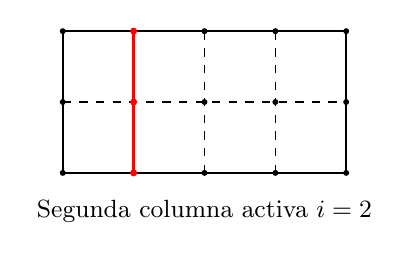
\begin{tikzpicture}[scale=0.45]
  \draw[thick] (0,0) rectangle (8,4);

  \foreach \j in {0,2,4} {
    \draw[thin,dashed] (0,\j) -- (8,\j);
  }
  \foreach \i in {0,2,4,6,8} {
    \draw[thin,dashed] (\i,0) -- (\i,4);
  }

  % Segunda columna activa i=2
  \draw[very thick,red] (2,0) -- (2,4);

  \foreach \i in {0,2,4,6,8} {
    \foreach \j in {0,2,4} {
      \fill (\i,\j) circle (2.4pt);
    }
  }
  \foreach \j in {0,2,4} {
    \fill[red] (2,\j) circle (2.8pt);
  }

  \node[below] at (4,-0.5) {\small Segunda columna activa \(i=2\)};
\end{tikzpicture}
\end{minipage}
\end{center}

An\'alogamente, para las otras columnas interiores:

\begin{equation}
\begin{aligned}
\mathbf r^{(y)}(i=3) &= [0,\,-5/7,\,0]^T,\\
\mathbf r^{(y)}(i=4) &= [0,\,-75/28,\,0]^T.
\end{aligned}
\end{equation}

Para cada \(i\in\{2,3,4\}\), el sistema vertical de tama\~no 3 usa:

\begin{equation}
\begin{aligned}
a^{(y)} &= [0,\;0.25,\;-1],\\
b^{(y)} &= [-1,\;-1,\;1],\\
c^{(y)} &= [1,\;0.25,\;0],
\end{aligned}
\end{equation}

y su factorizaci\'on:

\begin{equation}
\tilde c_1^{(y)}=-1,\quad \tilde c_2^{(y)}=-\frac13,\quad \tilde c_3^{(y)}=0,
\qquad
d_1^{(y)}=-1,\; d_2^{(y)}=-\frac34,\; d_3^{(y)}=\frac23.
\end{equation}

Tomando primero \(i=2\), con \(\mathbf r^{(y)}=[0,-5/28,0]^T\):

\begin{equation}
\begin{aligned}
\hat r_1 &= 0/(-1)=0,\\
\hat r_2 &= \frac{-5/28-0.25\cdot0}{-3/4}=\frac{5}{21},\\
\hat r_3 &= \frac{0-(-1)\hat r_2}{2/3}=\frac{3}{2}\hat r_2=\frac{5}{14},\\
t_3^{(y)} &= \hat r_3=\frac{5}{14},\\
t_2^{(y)} &= \hat r_2-\tilde c_2^{(y)}t_3^{(y)}
=\frac{5}{21}-\left(-\frac13\right)\frac{5}{14}=\frac{5}{14},\\
t_1^{(y)} &= \hat r_1-\tilde c_1^{(y)}t_2^{(y)}
=0-(-1)\frac{5}{14}=\frac{5}{14}.
\end{aligned}
\end{equation}

An\'alogamente, para \(i=3\) y \(i=4\):

\begin{equation}
\begin{aligned}
\mathbf{t}^{(y)}_{i=2} &= [5/14,\;5/14,\;5/14]^T,\\
\mathbf{t}^{(y)}_{i=3} &= [10/7,\;10/7,\;10/7]^T,\\
\mathbf{t}^{(y)}_{i=4} &= [75/14,\;75/14,\;75/14]^T.
\end{aligned}
\end{equation}

Al finalizar la primera iteraci\'on completa (barrido \(x\) y barrido \(y\)), el
campo queda:

\begin{equation}
T^{(1)} =
\begin{bmatrix}
0 & 5/14 & 10/7 & 75/14 & 0 \\
0 & 5/14 & 10/7 & 75/14 & 10 \\
0 & 5/14 & 10/7 & 75/14 & 0
\end{bmatrix},
\end{equation}

Finalmente, el residuo que usa el programa es:

\begin{equation}
R^{(1)} =
\left[
\sum_{i=1}^{5}\sum_{j=1}^{3}
\left(T_{i,j}^{(1)}-T_{i,j}^{(0)}\right)^2
\right]^{1/2}
\approx 13.88,
\end{equation}

valor muy superior a la tolerancia, por lo que el ciclo iterativo contin\'ua.

\medskip

A continuaci\'on se explica la implementaci\'on computacional del algoritmo 
secuencial para el caso 2D.

\section{Metodolog\'ia computacional secuencial del caso 2D}

El algoritmo secuencial para el caso 2D se implementa en el programa 
\texttt{secuencial/calor2D/calor2D.f90} y
\texttt{secuencial/calor2D/tridiagonal.f90}. Se resuelve iterativamente el 
sistema de ecuaciones generado por la discretización bidimensional de la 
ecuación de Laplace. Se usa el mismo algoritmo de Thomas para resolver los 
sistemas tridiagonales en cada dirección. El programa se ejecuta con 
\verb|./calor2D| y los resultados se guardan en archivos de texto para su 
posterior análisis.

\medskip

Se comienza con la implementación del programa principal \texttt{Calor2D.f90}, 
donde se declaran las variables y los parámetros necesarios para la simulación.

\begin{verbatim}
  Program Calor2D
  !
  Implicit none
  !
  ! Declaraci\'on de variables
  !
  ! Iteradores y tamaño del problema
  !
  integer :: ii, jj, iter
  integer, parameter :: nx = 60, ny = 30, itermax=10000
  !
\end{verbatim}

Seguidamente, se inicializan los parámetros del dominio computacional, 
incluyendo las dimensiones del dominio $L_x$ y $L_y$, los pasos de malla 
$\Delta x$ y $\Delta y$, y los inversos de los cuadrados de los pasos para 
optimizar los cálculos.

\begin{verbatim}
  ! Variables del dominio computacional
  !
  double precision :: lx, ly, deltax, deltay
  double precision :: inv_dx2, inv_dy2
  !
  ! Variable para el residuo de iteraciones, y tolerancia
  !
  double precision :: residuo, tolerancia, tolerancia2
\end{verbatim}

Las variables del problema físico incluyen el vector de incógnitas $tt$ para 
almacenar las temperaturas en cada iteración, los vectores $tx$ y $ty$ para 
almacenar las temperaturas en cada dirección, los vectores $rx$ y $ry$ para 
almacenar los resultados de los sistemas de ecuaciones, y los vectores $cfx$ y 
$cfy$ para almacenar las condiciones de frontera.

\begin{verbatim}
  !
  ! Variables del problema f\'isico
  !
  double precision :: tt(nx,ny,2)     ! vector de inc\'ognitas, 1 para la iteraci\'on actual 
                                      ! y 2 para la anterior
  double precision :: tx(nx), ty(ny)  ! vectores de inc\'ognitas 1D
  double precision :: rx(nx),ry(ny)   ! vector de resultados del s. ecuaciones
  double precision :: cfx(ny,2),cfy(nx,2) ! vector de condiciones de frontera
\end{verbatim}

Asimismo, se necesita de una matriz tridiagonal sobredimensionada para cada direcci\'on
para almacenar los coeficientes de los sistemas tridiagonales. En este caso, se opta por usar 
vectores separados para cada dirección, lo que permite una implementación más 
clara y eficiente del algoritmo de Thomas para resolver los sistemas 
tridiagonales en cada dirección. Estos vectores se declaran para
almacenar los coeficientes de los sistemas tridiagonales en cada dirección. 
Se declaran los vectores $ax$, $bx\_base$ y $cx$ para la dirección $x$, y los 
vectores $ay$, $by\_base$ y $cy$ para la dirección $y$. Además, se declaran los 
vectores $cpx$, $denx$, $cpy$ y $deny$ para almacenar la factorización de Thomas.

\begin{verbatim}
  !
  ! Variables para almacenar los coeficientes de los sistemas tridiagonales
  !
  double precision :: ax(nx), cx(nx), bx_base(nx) ! Variables para almacenar
  !                                               ! matriz tridiagonal sobredimensionada
  double precision :: cpx(nx), denx(nx)
  !
  double precision :: ay(ny), cy(ny), by_base(ny) ! Variables para almacenar
  !                                               ! matriz tridiagonal sobredimensionada
  double precision :: cpy(ny), deny(ny)
\end{verbatim}

A continuación, se establecen los parámetros de la simulación, incluyendo la 
tolerancia para la convergencia y las dimensiones del dominio computacional. 
Se calculan los pasos de malla y los inversos de los cuadrados de los pasos 
para optimizar los cálculos en el algoritmo de Thomas.

\begin{verbatim}
  !
  ! Tolerancia
  !
  tolerancia = 1d-3
  tolerancia2 = tolerancia*tolerancia
  !
  ! Dominio computacional
  !
  lx      = 10.d0
  deltax  = lx/(nx - 1) ! nx puntos definen (nx - 1) intervalos
  ly      = 5.d0
  deltay  = ly/(ny - 1) ! ny puntos definen (ny - 1) intervalos
  inv_dx2 = 1.d0/(deltax*deltax)
  inv_dy2 = 1.d0/(deltay*deltay)
\end{verbatim}

Se realiza la inicializaci\'on de los vectores de coeficientes y del campo de 
temperaturas. Todos los vectores de coeficientes $a_x$, $b_x$, $c_x$ para la 
direcci\'on $x$ y $a_y$, $b_y$, $c_y$ para la direcci\'on $y$, así como los 
vectores de t\'erminos independientes $r_x$ y $r_y$. 

\medskip

Se crean los vectores \texttt{ax}, \texttt{bx\_base}, \texttt{cx}, etc, que 
se ir\'an llenando con los coeficiente de las matrices tridiagonales para cada 
direcci\'on seg\'un las ecuaciones \ref{eq:coef_tridiagonal_x_2D_a} - 
\ref{eq:coef_tridiagonal_x_2D_c} y \ref{eq:coef_tridiagonal_y_2D_a} - 
\ref{eq:coef_tridiagonal_y_2D_c}. El campo de temperatura $T(i,j,n)$ también se inicializa a cero, pudiendo 
modificarse posteriormente para establecer condiciones iniciales espec\'ificas:

\begin{verbatim}
  !
  ! Inicializacion de variables
  !
  ax(:)   = 0.d0
  bx_base(:) = 0.d0
  cx(:)   = 0.d0
  rx(:)   = 0.d0
  ay(:)   = 0.d0
  by_base(:) = 0.d0
  cy(:)   = 0.d0
  ry(:)   = 0.d0
  tt(:,:,:) = 0.d0 ! Valores iniciales de temperatura, se pueden modificar 
                   ! para probar diferentes condiciones iniciales
  !
  ! Coeficientes constantes de los sistemas tridiagonales.
  !
  do ii = 2, nx-1
     ax(ii) = inv_dx2
     bx_base(ii) = -2.d0*(inv_dx2 + inv_dy2)
     cx(ii) = inv_dx2
  end do
  ax(1) = 0.d0
  bx_base(1) = 1.d0
  cx(1) = 0.d0
  ax(nx) = 0.d0
  bx_base(nx) = 1.d0
  cx(nx) = 0.d0
  !
  do jj = 2, ny-1
     ay(jj) = inv_dy2
     by_base(jj) = -2.d0*(inv_dx2 + inv_dy2)
     cy(jj) = inv_dy2
  end do
  ay(1) = 0.d0
  by_base(1) = -1.d0
  cy(1) = 1.d0
  ay(ny) = -1.d0
  by_base(ny) = 1.d0
  cy(ny) = 0.d0
\end{verbatim}

Ya que los coeficientes tridiagonales (a, b, c) son constantes durante todas las
iteraciones, se pueden calcular una sola vez y almacenar en las operaciones de 
factorizaci\'on con \texttt{tri\_factor}.

\begin{verbatim}
  !
  call tri_factor(ax,bx_base,cx,cpx,denx,nx)
  call tri_factor(ay,by_base,cy,cpy,deny,ny)
\end{verbatim}

Asimismo, se est\'a resolviendo una placa bidimensional, las condiciones 
frontera se expresar\'an como vectores para cada direcci\'on. 
En este caso, se trabaja con condiciones mixtas: Dirichlet en direcci\'on $x$
y Neumann homog\'enea en direcci\'on $y$. En $x$ se fija la temperatura en los
dos bordes ($T=1^{o}C$ a la izquierda y $T=0^{o}C$ a la derecha), mientras que en $y$
se impone flujo nulo en ambos extremos ($\partial T/\partial y = 0$). Esto se
traduce en 

\begin{equation}
  \begin{array}{l}
    cfx_1 = T_0 = 1, \quad cfy_1 = -k \frac{\partial T}{\partial y}\bigg|_{y=0} = 0, \\
    cfx_{2} = T_{L_x} = 0, \quad cfy_{2} = -k \frac{\partial T}{\partial y}\bigg|_{y=L_y} = 0.
  \end{array}
\end{equation}

Donde, para la direcci\'on $x$, se fija $T=1^{o}C$ en el borde izquierdo y
$T=0^{o}C$ en el borde derecho.

\medskip

Las 4 condiciones frontera se almacenan en los vectores \texttt{$cfx$} 
y \texttt{$cfy$} para cada direcci\'on. As\'i,

\begin{equation}
  \begin{array}{l}
    cfx(i,1) = 1, \quad cfx(i,2) = 0 \quad \forall i \in [1, n_x], \\
    cfy(j,1) = 0, \quad cfy(j,2) = 0 \quad \forall j \in [1, n_y]
  \end{array}
\end{equation}

\begin{verbatim}
  !
  ! Condiciones de frontera en direcci'on x
  !
  do ii = 1, ny
     cfx(ii,1) = 1.d0
     cfx(ii,2) = 0.d0
  end do
  !
  ! Condiciones de frontera en direcci'on y
  !
  do jj = 1, nx
     cfy(jj,1) = 0.d0
     cfy(jj,2) = 0.d0
  end do
\end{verbatim}

Luego, se ejecuta el bucle de iteraciones para resolver el sistema de 
ecuaciones. En cada iteración, se actualiza el valor de la iteración anterior, 
se ensamblan los sistemas tridiagonales para cada dirección y se resuelven 
usando el algoritmo de Thomas. El proceso se repite hasta alcanzar la 
convergencia o el número máximo de iteraciones.

\medskip

Se  comienza respaldando el valor de la iteraci\'on anterior en 
\texttt{tt(:,:,2)} para poder calcular el residuo posteriormente. Luego, se 
realiza el barrido en la direcci\'on $y$ y dentro de este, el barrido en la 
direcci\'on $x$ para ensamblar los sistemas tridiagonales correspondientes a 
cada línea horizontal $j$.

\begin{verbatim}
  bucle_iteraciones: do iter = 1, itermax
     !
     ! Inicializamos el valor de la iteraci'on anterior
     !
     tt(:,:,2) = tt(:,:,1)
     !
     barrido_y: do jj = 2, ny-1
        ensambla_tri_x: do ii = 2, nx-1

           rx(ii) = -inv_dy2*tt(ii,jj-1,1) - inv_dy2*tt(ii,jj+1,1)
           
        end do ensambla_tri_x
\end{verbatim}

El vector \texttt{rx} se llena seg\'un la ecuaci\'on 
\ref{eq:coef_tridiagonal_x_2D_r} para cada nodo interior. Sus valores frontera
se imponen seg\'un las condiciones de frontera almacenadas en \texttt{cfx}.

\begin{verbatim}
        !
        ! Impone cond. frontera
        !
        rx(1)     = cfx(jj,1)
        !
        rx(nx)    = cfx(jj,2)
        !
        ! Resolver el problema algebraico
        !
        call tri_solve(ax,cpx,denx,rx,tx,nx)
        !
        ! Actualizar la temperatura de la placa
        !
        do ii = 1, nx
           
           tt(ii,jj,1) = tx(ii)
           
        end do
        !
     end do barrido_y
\end{verbatim}

  Luego se realiza el barrido complementario en la direcci\'on \texttt{x}. En
  este caso, para cada columna interior \(i\), se ensambla el sistema
  tridiagonal en \texttt{y} usando la ecuaci\'on
  \ref{eq:coef_tridiagonal_y_2D_r}. Despu\'es se imponen las fronteras con
  \texttt{cfy}, se resuelve el sistema y se actualiza la columna completa
  \texttt{tt(ii,jj,1)}.

  \begin{verbatim}
      barrido_x: do ii = 2, nx-1
        ensambla_tri_y: do jj = 2, ny-1

          ry(jj) = -inv_dx2*tt(ii-1,jj,1) - inv_dx2*tt(ii+1,jj,1)

        end do ensambla_tri_y
        !
        ! Impone cond. frontera
        !
        ry(1)     = cfy(ii,1)
        !
        ry(ny)    = cfy(ii,2)
        !
        ! Resolver el problema algebraico
        !
        call tri_solve(ay,cpy,deny,ry,ty,ny)
        !
        ! Actualizar la temperatura de la placa
        !
        do jj = 1, ny

          tt(ii,jj,1) = ty(jj)

        end do
        !
      end do barrido_x
  \end{verbatim}

  Con ambos barridos completados, el programa eval\'ua la convergencia mediante
  el residuo cuadr\'atico entre la iteraci\'on actual y la anterior. El residuo
  se acumula sobre todos los nodos y se compara con
  \texttt{tolerancia2 = tolerancia*tolerancia}. Si el residuo es menor que ese
  umbral, se sale del bucle iterativo.

  \begin{verbatim}
      !
      ! Criterio de convergencia
      !
      residuo = 0.d0
      do jj = 1, ny
        do ii = 1, nx
          residuo = residuo + (tt(ii,jj,1)-tt(ii,jj,2))*(tt(ii,jj,1)-tt(ii,jj,2))
        end do
      end do
      !
      if( residuo < tolerancia2 )exit
      !
    end do bucle_iteraciones
  \end{verbatim}

  Finalmente, al terminar el proceso iterativo, se reporta el n\'umero de
  iteraciones y se escribe el campo de temperatura en formato
  \((x,y,T)\), separando visualmente cada fila de \(y\) con una l\'inea en blanco.

  \begin{verbatim}
    write(*,*) "Convergencia en ", iter, " iteraciones"
    !
    do jj = 1, ny
      do ii = 1, nx
        write(*,*) (ii-1)*deltax, (jj-1)*deltay, tt(ii,jj,1)
      end do
      write(*,*) ' '
    end do
    !
  end Program Calor2D
  \end{verbatim}

\section{Caso 2D paralelo con OpenMP} 
La versi\'on paralela distribuye los barridos independientes entre hilos de
OpenMP. Si $t_p$ es el tiempo de ejecuci\'on usando $p$ hilos y $t_1$ es el
tiempo de referencia secuencial, el speedup se calcula como:

\begin{equation}
S_p=\frac{t_1}{t_p}.
\end{equation}

La eficiencia paralela mide qu\'e fracci\'on del uso ideal de los $p$ hilos se
aprovecha:

\begin{equation}
E_p=\frac{S_p}{p}.
\end{equation}

El caso ideal corresponde a:

\begin{equation}
S_p^{ideal}=p,
\quad
E_p^{ideal}=1.
\end{equation}

\section{Resultados}

Las tablas de rendimiento se guardan en \texttt{docs/tables/} y las figuras en
\texttt{docs/figures/}. Para cada n\'umero de hilos $p$, el tiempo reportado se
puede obtener como el promedio de varias corridas:

\begin{equation}
\overline{t}_p=\frac{1}{N}\sum_{\ell=1}^{N}t_{p,\ell},
\end{equation}

donde $N$ es el n\'umero de repeticiones y $t_{p,\ell}$ es el tiempo medido en
la corrida $\ell$ usando $p$ hilos. Con este promedio, el speedup experimental
queda:

\begin{equation}
S_p^{real}=\frac{\overline{t}_1}{\overline{t}_p}.
\end{equation}

La eficiencia experimental se calcula como:

\begin{equation}
E_p^{real}=\frac{S_p^{real}}{p}
=\frac{\overline{t}_1}{p\,\overline{t}_p}.
\end{equation}

Para comparar con la aceleraci\'on ideal se usa:

\begin{equation}
\Delta S_p = S_p^{ideal}-S_p^{real}=p-S_p^{real}.
\end{equation}

Una diferencia $\Delta S_p$ cercana a cero indica que la ejecuci\'on paralela se
aproxima al comportamiento ideal. Cuando $\Delta S_p$ crece, la eficiencia baja
por costos de sincronizaci\'on, acceso a memoria, regiones no paralelas o
desbalance entre hilos.

\subsection{Comparaci\'on final con el c\'odigo de referencia}

Se compar\'o la versi\'on paralela desarrollada en \texttt{paralelo/src/} contra
el c\'odigo de referencia proporcionado en \texttt{paralelo/reference/}. Los
archivos de referencia no fueron modificados. Para reducir el efecto de
arranques fr\'ios y procesos de fondo, se us\'o una corrida de calentamiento por
n\'umero de hilos y se report\'o la mediana de seis corridas medidas.

Para aislar el efecto del paralelismo bajo el mismo comportamiento num\'erico,
en la versi\'on desarrollada se reprodujeron dos errores presentes en
\texttt{reference/}: (i) la condici\'on de frontera inferior del barrido en
direcci\'on $y$ se dej\'o con la misma formulaci\'on incorrecta, y (ii) el corte
por convergencia basado en residuo se mantuvo desactivado, forzando la
ejecuci\'on hasta \texttt{itermax}.

La comparaci\'on debe leerse como una comparaci\'on de comportamiento paralelo en
la misma m\'aquina, no como igualdad estricta de carga num\'erica: ambas versiones 
usan una malla de $480\times 240$.

\begin{table}[H]
\centering
\caption{Comparaci\'on de tiempos y aceleraci\'on en la misma m\'aquina.}
\label{tab:comparacion-speedup-final}
\begin{tabular}{rrrrr}
\toprule
Hilos & $t_{\mathrm{nuestra}}$ [s] & $S_{\mathrm{nuestra}}$ &
$t_{\mathrm{ref}}$ [s] & $S_{\mathrm{ref}}$ \\
\midrule
1 & 40.466 & 1.000 & 36.954 & 1.000 \\
2 & 21.829 & 1.854 & 21.855 & 1.691 \\
3 & 15.465 & 2.617 & 15.736 & 2.348 \\
4 & 13.534 & 2.990 & 14.136 & 2.614 \\
5 & 12.845 & 3.150 & 10.911 & 3.387 \\
6 & 11.342 & 3.568 &  9.832 & 3.759 \\
7 &  8.554 & 4.731 &  8.890 & 4.157 \\
8 &  8.102 & 4.994 & 10.386 & 3.558 \\
\bottomrule
\end{tabular}
\end{table}

\begin{figure}[H]
\centering
\includegraphics[width=0.78\textwidth]{comparacion_speedup_final.png}
\caption{Curvas de aceleraci\'on de la versi\'on desarrollada y la referencia.}
\label{fig:comparacion-speedup-final}
\end{figure}


\section{Conclusiones}



\bibliographystyle{plain}
\bibliography{bib/references}

\end{document}
